\chapter{Sorting association rules with \capa}
\label{chap:capa}


\minitoc


Although item-centric mining with \toppi provides an intuitive organization of each item's associations,
its ranking by decreasing frequency does not always select the most interesting ones ---
see the discussion in Section~\ref{sec:toppi:stars}.
Existing work proposes many functions to %(we implement \nbm of them)
measure the quality of association rules without additional knowledge~\cite{GengACM06,Lenca2007}.
However, we cannot know from existing studies which measure is able to
assign top rankings to significant associations in the retail domain.

In this chapter, we want to perform targeted analytics over the 3 \datalyse mining scenarios,
described in Section~\ref{sec:scenarios} (p.\pageref{sec:scenarios}).
The analyst provides input items or product categories of interest,
and expects the system to directly highlight a few dozen results.
This is very common in the marketing domain,
when checking the impact of advertisement operations or evaluating their opportunity.
As the analyst not only provides a non-negligible frequency threshold,
but also one or more conditions on the itemsets to be generated,
the computation is tractable on our datasets.
%The ability to identify valuable association rules is therefore
%of the utmost importance to avoid drowning analysts in useless information.
Still, it generates a very high number of rules, typically in the order of millions.

Building a system able to highlight automatically interesting associations
therefore raises two questions:

\begin{itemize}
  \item when sorting association rules,
    how different are the top results proposed by quality measures proposed in the literature?

  \item which quality measure(s) highlights association rules of the greatest interest to retail analysts?
\end{itemize}

In this chapter we address these questions with the following contributions:

\begin{itemize}
  \item We present in Section~\ref{sec:capa} \capa (Comparative Analysis of PAtterns),
    a framework to compare rule rankings produces by \nbm interestingness measures~\cite{GengACM06,Lenca2007}.% applied to association rules generated in the food retail domain.
    %In , we start by presenting \capa's components and how
    %it is integrated in our analytics workflow.

  \item We automatically compare the \nbm rankings in Section~\ref{sec:xp:empirical},
    and distinguish 5 groups of similar measures.%, regardless of the mining scenario.

  \item For this automatic evaluation we introduce a new ranking similarity measure:
    Normalized Discounted Correlation Coefficient ({\em NDCC}).
    %{\em NDCC} bridges the gap between taking into account all rules in the two rankings being compared,
    %and only considering the top-$k$ ones.
%that draws inspiration from Normalized Discounted Cumulative Gain~\cite{JarvelinACM02},
%a commonly used ranking comparison in Information Retrieval.

  \item We conduct a user study with two experienced domain experts from Intermarch\'e, in Section~\ref{sec:xp:user},
    in order to evaluate which of our 5 groups of interestingness measures are meaningful in their domain.
\end{itemize}



We conclude in Section~\ref{sec:capa:conc}.


%\pagebreak


\section{The \capa framework}
\label{sec:capa}

Looking back at our complete workflow (depicted p.\pageref{fig:archoverview})
\capa belongs to the mining and exploitation steps.
We start by describing and motivating how each step is implemented and integrated in our system.

Our goal is to enable analysts to test and compare different interestingness measures
on a set of transactions $\cal D$ produced by our curation module.
Thus an analyst firstly specifies one of our 3 mining scenarios (\demoassoc, \prodassocreceipt or \prodassocclient)
and a minimum support threshold $\varepsilon$.
When using \capa analysts focus on one or several targets:
categories in the case of \demoassoc, products in the case of the other two.
Thus, in addition to the common model for itemset mining presented in
Section~\ref{sec:model:mining} (p.\pageref{sec:model:mining}),
\capa also requires the definition of a {\em target items} set ${\cal B} \subset {\cal I}$.
Once these settings are determined,
the system generates a list of association rules ranked using different interestingness measures.

In Section~\ref{sec:capa:intro} we show that different quality measures from the literature
can highlight very different association rules.
We also detail the \nbm measures implemented in \capa and the data needed for our rankings comparison.
\capa mines association rules whose consequent side is a single target item from ${\cal B}$:
Section~\ref{sec:capa:mining} shows how we modify \jlcm to mine this finer set of association rules,
and the post-processing step which provides enough data to compute each quality measure for each rule.
Section~\ref{sec:capa:exploit} then describes the exploitation step of \capa,
{\em ie.} how associations are ranked and presented to the analyst.

\subsection{Different measures highlight different rules}
\label{sec:capa:intro}

As discussed in Section~\ref{sec:lcm} (p.\pageref{sec:lcm}),
given a frequency threshold $\varepsilon$
we can find all frequent CIS with \jlcm
and use them to derive association rules.
Association rules were originally selected using thresholds for support and confidence~\cite{AgrawalSIGMOD93}.
However, support and confidence do not always coincide with the interest of analysts.
Setting thresholds is also not easy and may not be sufficient to filter results.
%When the goal is to rank rules, using two separate values is not natural.
For example, in the \demoassoc case, using a minimum support of \num{1000} \jlcm mines \num{2746418}
frequent rules of the form {\em customer segment} $\rightarrow$ {\em product category}.
Out of these, \num{15063} have a confidence of $50\%$ or higher.
Hence a number of interestingness measures that serve different analyses needs
were proposed in the literature~\cite{GengACM06,Lenca2007}.

\begin{table}
  %\setlength{\tabcolsep}{2pt}
	\begin{tabular}{cc}
		\begin{subtable}[b]{0.48\textwidth}
      \begin{tabular}{|rl|}
      \hline
      \multicolumn{2}{|c|}{\textbf{by confidence}}               \\\hline
      $\{> 65, F, $ Aube$\}$&$\rightarrow$ {\em Dairy}       \\
      $\{> 65, F, $ Aveyron$\}$&$\rightarrow$ {\em Dairy}       \\
      $\{> 65, F, $ Val de Marne$\}$& $ \rightarrow$ {\em Dairy}       \\
      $\{> 65, F, $ Seine S$^{t}$ Denis$\}$& $ \rightarrow$ {\em Dairy}       \\
      $\{> 65, F, $ Haute Saone$\}$& $ \rightarrow$ {\em Dairy}       \\
      $\{> 65, F, $ Meuse$\}$& $ \rightarrow$ {\em Dairy}       \\
      $\{> 65, *, $ Aube$\}$& $ \rightarrow$ {\em Dairy}       \\
      $\{> 65, F, $ Haute Vienne$\}$& $ \rightarrow$ {\em Dairy}       \\
      $\{> 65, F, $ Maine et Loire$\}$& $ \rightarrow$ {\em Dairy}       \\
      $\{> 65, *, $ Val de Marne$\}$& $ \rightarrow$ {\em Dairy}           \\\hline
      \end{tabular}
		\end{subtable}
		&
		\hfill
		\begin{subtable}[b]{0.48\textwidth}
      \begin{tabular}{|rl|}
      \hline
      \multicolumn{2}{|c|}{\textbf{by Piatetsky-Shapiro~\cite{PiatetskyKDD91}}}       \\\hline
    $\{*, *, $ Nord$\}$&$\rightarrow$ {\em Liquids}       \\
    $\{*, *, $ Nord$\}$&$\rightarrow$ {\em Soft drinks}       \\
    $\{*, *, $ Nord$\}$&$\rightarrow$ {\em Beers}       \\
    $\{*, *, $ Nord$\}$&$\rightarrow$ {\em Spreads}       \\
    $\{*, F, $ Nord$\}$&$\rightarrow$ {\em Soft drinks}       \\
    $\{*, *, $ Nord$\}$&$\rightarrow$ {\em Imported beers}       \\
    $\{*, F, $ Nord$\}$&$\rightarrow$ {\em Liquids}       \\
    $\{*, F, $ Nord$\}$&$\rightarrow$ {\em Beers}       \\
    $\{*, *, $ Finistere$\}$&$\rightarrow$ {\em Butters}       \\
    $\{*, F, $ Garonne$\}$&$\rightarrow$ {\em Drugstore}          \\\hline
    \end{tabular}
		\end{subtable}
		\\
		\begin{subtable}{0.48\textwidth}
  		\vspace{1em}
      \begin{tabular}{|rl|}
      \hline
      \multicolumn{2}{|c|}{\textbf{by Pearson's $\chi^2$}}      \\\hline
      $\{*, *, $ Somme$\}$&$\rightarrow$ {\em Cut cheese}       \\
       $\{*, F, $ Somme$\}$&$\rightarrow$ {\em Cut cheese}       \\
      $\{> 65, *,$ Morbihan$\}$&$\rightarrow$ {\em Fresh milk}       \\
      $\{> 65, *,$ Somme$\}$&$\rightarrow$ {\em Cut cheese}       \\
      $\{*, *,$ Finistere$\}$&$\rightarrow$ {\em Canned pork}       \\
      $\{*, *,$ Cotes\ d'Armor$\}$&$\rightarrow$ {\em Canned pork}       \\
      $\{> 65, F,$ Morbihan$\}$&$\rightarrow$ {\em Fresh milk}       \\
      $\{*, *,$ Nord$\}$&$\rightarrow$ {\em Beer}       \\
      $\{*, *,$ Nord$\}$&$\rightarrow$ {\em Sparkling liquors}       \\
      $\{*, *,$ Vienne$\}$&$\rightarrow$ {\em Breakfast biscuits}   \\\hline
      \end{tabular}
		\end{subtable}
		&
		\hfill
		\begin{minipage}{0.32\linewidth}
  		\vspace{1em}
			\caption{\label{tab:eyecatcher}
        Top-10 demographics association rules, according to different interestingness measures.
        Rules are denoted $\{\mathit{age, gender, department}$ $\} \rightarrow$ {\em product category}.
        Product categories were translated to English for clarity.
        French departments were left unchanged.
      }
		\end{minipage}
		\\
	\end{tabular}
\end{table}


Table~\ref{tab:eyecatcher} shows a ranking of the top-10 rules
according to 3 different interestingness measures proposed in ~\cite{GengACM06}.
If we denote rules as $A \rightarrow B$,
{\em confidence} is the probability to observe $B$ given that we observed $A$, i.e., $P(B|A)$.
{\em Piatetsky-Shapiro}~\cite{PiatetskyKDD91} measures the difference
between the probability to observe $A$ and $B$ together
and the expected probability assuming they are independent,  i.e., $P(AB) - P(A)P(B)$.
{\em Pearson's} $\chi^2$, measures how unlikely observations of $A$ and $B$ are independent.
Clearly, these measures highlight very different associations.


% !TEX root = ../paper.tex

\begin{table}[H]
{\footnotesize
  \centering
  \begin{tabular}{|l|l|c|}
		\hline
    \textbf{Measure}  &   \textbf{Formula} &\textbf{Group}\\\specialrule{.15em}{0em}{0em}
    One-Way Support                  & $P(B|A)\times log_{2}\frac{P(AB)}{P(A)P(B)}$ &\cellcolor{g1aColor}\\\cline{1-2}
    Relative Risk                    & $P(B|A) / P(B|\neg A)$ &\cellcolor{g1aColor}\\\cline{1-2}
    Odd Multiplier                   & $\frac{P(AB)P(\neg B)}{P(B)P(A \neg B)}$ &\cellcolor{g1aColor}\\\cline{1-2}
    Zhang                            & $\frac{P(AB)-P(A)P(B)}{max(P(AB)P(\neg B), P(B)P(A \neg B))}$ &\cellcolor{g1aColor}\\\cline{1-2}
    Yule's Q $\Diamond$                        & $\frac{P(AB)P(\neg A \neg B)-P(A \neg B)P(B \neg A)}{P(AB)P(\neg A \neg B)+P(A \neg B)P(B \neg A)}$ &\cellcolor{g1aColor}\\\cline{1-2}
    Yule's Y $\Diamond$                        & $\frac{\sqrt{P(AB)P(\neg A \neg B)}-\sqrt{P(A \neg B)P(B \neg A)}}{\sqrt{P(AB)P(\neg A \neg B)}+\sqrt{P(A \neg B)P(B \neg A)}}$ &\cellcolor{g1aColor}\\\cline{1-2}
    Odds Ratio $\Diamond$                      & $\frac{P(AB)P(\neg A \neg B)}{P(A \neg B)P(B \neg A)} $ &\cellcolor{g1aColor}\\\cline{1-2}
    Information Gain $\ast$$\ominus$          & $\mathit{log}(P(AB)/(P(A)P(B)))$ &\cellcolor{g1aColor}\\\cline{1-2}
    Lift $\ast$$\ominus$                            & $P(AB)/(P(A)P(B))$&\cellcolor{g1aColor}\\\cline{1-2}
    Bayes Factor $\ast$                    & $P(A|B)/P(A|\neg B)$ & \cellcolor{g1aColor}\multirow{-9}{*}{$G_1^a$} \\\specialrule{.12em}{0em}{0em}
%
    Added Value $\ast$                     & $P(B|A) - P(B)$ &\cellcolor{g1bColor}\\\cline{1-2}
    Certainty Factor $\ast$                & $(P(B|A) - P(B)) / (1 - P(B))$ &\cellcolor{g1bColor}\\\cline{1-2}
    Confidence $\ast$$\otimes$          & $P(B|A)$ &\cellcolor{g1bColor}\\\cline{1-2}
    Centered Confidence $\ast$             & $P(B|A) - P(B)$  &\cellcolor{g1bColor}\\\cline{1-2}
    Loevinger $\dagger$                       & $1 - \frac{P(A)P(\neg B)}{P(A \neg B)}$ &\cellcolor{g1bColor}\\\cline{1-2}
    Conviction $\dagger$                      & $\frac{P(A)P(\neg B)}{P(A \neg B)}$ &\cellcolor{g1bColor}\\\cline{1-2}
    \pbox{10cm}{Examples and Counter-\\examples Rate} & $1 - \frac{P(A \neg B)}{P(AB)}$ &\cellcolor{g1bColor}\\\cline{1-2}
    Sebag-Schoenauer                 & $\frac{P(AB)}{P(A \neg B)}$ &\cellcolor{g1bColor}\\\cline{1-2}
    Leverage                         & $P(B|A) - P(A)P(B)$ &\cellcolor{g1bColor}\\\cline{1-2}
    Laplace Correction $\ast$$\otimes$          & $\frac{\mathit{support}(AB)+1}{\mathit{support}(A)+2}$  & \cellcolor{g1bColor}\multirow{-9}{*}{$G_1^b$}\\\specialrule{.15em}{0em}{0em}
%%
    Least Contradiction              & $\frac{P(AB)-P(A \neg B)}{P(B)}$ &\cellcolor{g2Color}\\\cline{1-2}
    Accuracy                         & $P(AB) + P(\neg A \neg B)$ &\cellcolor{g2Color}\multirow{-2}{*}{$G_2$}\\\specialrule{.15em}{0em}{0em}
%%
    Pearson's $\chi^2$ $\triangleright$              & $|{\cal T}| \times \left(\frac{(P(AB)-P(A)P(B))^2}{P(A)P(B)} + \frac{(P(\neg A B)-P(\neg A)P(B))^2}{P(\neg A)P(B)}\right)$&\cellcolor{g3Color}\\
&$+ |{\cal T}| \times \left(\frac{(P(A \neg B)-P(A)P(\neg B))^2}{P(A)P(B)} + \frac{(P(\neg A \neg B)-P(\neg A)P(\neg B))^2}{P(\neg A)P(\neg B)}\right)$&\cellcolor{g3Color}\\\cline{1-2}
    Gini Index $\triangleright$                      & $P(A)\times(P(B|A)^2 + P(\neg B|A)^2) + P(\neg A)\times(P(B|\neg A)^2+$&\cellcolor{g3Color}\\
&$P(\neg B|\neg A)^2)-P(B)^2 - P(\neg B)^2$&\cellcolor{g3Color}\\\cline{1-2}
    J-measure                        & $P(AB)log(\frac{P(B|A)}{P(B)})+P(A \neg B)log(\frac{P(\neg B|A)}{P(\neg B)})$ &\cellcolor{g3Color}\\\cline{1-2}
    \pbox{10cm}{$\Phi$ Linear Correlation \\Coefficient} & $\frac{P(AB)-P(A)P(B)}{\sqrt{P(A)P(B)P(\neg A)P(\neg B)}}$&\cellcolor{g3Color}\\\cline{1-2}
    Two-Way Support         & $P(AB)\times log_{2}\frac{P(AB)}{P(A)P(B)} + P(A \neg B)\times log_{2}\frac{P(A \neg B)}{P(A)P(\neg B)} +$ &\cellcolor{g3Color}\\
    Variation        & $P(\neg A B)\times log_{2}\frac{P(\neg A B)}{P(\neg A)P(B)} + P(\neg A \neg B)\times log_{2}\frac{P(\neg A \neg B)}{P(\neg A)P(\neg B)}$&\cellcolor{g3Color}\\\cline{1-2}
    Fisher's exact test               & $\frac{\binom{|{\cal T}|\times P(B)}{|{\cal T}| \times P(AB)}\binom{|{\cal T}| \times P(\neg B)}{|{\cal T}| \times P(A\neg B)}}{\binom{|{\cal T}|}{|{\cal T}|\times P(A)}}$ &\cellcolor{g3Color}\\\cline{1-2}
    Jaccard                          & $P(AB) / (P(A)+P(B)-P(AB))$ &\cellcolor{g3Color}\\\cline{1-2}
    Cosine                           & $\frac{P(AB)}{\sqrt{P(A)P(B)}}$ &\cellcolor{g3Color}\\\cline{1-2}
    Implication Index                & $\frac{\mathit{support}(A)\mathit{support}(B)-|{\cal T}|\mathit{support}(AB)}{\sqrt{|{\cal T}|\mathit{support}(A)\mathit{support}(\neg B)}}$ & \cellcolor{g3Color} \\\cline{1-2}
    Kappa Coefficient                & $2\frac{|{\cal T}|\mathit{support}(AB)-\mathit{support}(A)\mathit{support}(B)}{|{\cal T}|\mathit{support}(A)+|{\cal T}|\mathit{support}(B)-2\mathit{support}(A)\mathit{support}(B)}$ &
      \cellcolor{g3Color}\multirow{-13}{*}{$G_3$} \\
      \specialrule{.15em}{0em}{0em}
%%
    Two-Way Support                  & $P(AB)\times log_{2}\frac{P(AB)}{P(A)P(B)}$&\cellcolor{g4Color}\\\cline{1-2}
    Piatetsky-Shapiro                & $P(AB)-P(A)P(B)$ &\cellcolor{g4Color}\\\cline{1-2}
    Klosgen                          & $\sqrt{P(AB)}\mathit{max}(P(B|A)-P(B), P(A|B)-P(A))$ &\cellcolor{g4Color}\\\cline{1-2}
    Specificity                      & $P(\neg B | \neg A)$ &\cellcolor{g4Color}\multirow{-4}{*}{$G_4$}\\\specialrule{.15em}{0em}{0em}
%%
    Recall                           & $P(A|B)$ &\cellcolor{g5Color}\\\cline{1-2}
    Collective Strength              & $\frac{P(AB)+P(\neg B|\neg A)}{P(A)P(B)+P(\neg A)P(\neg B)}\times\frac{1-P(A)P(B)-P(\neg A)P(\neg B)}{1 - P(AB) - P(\neg B|\neg A)}$&\cellcolor{g5Color}\multirow{-2}{*}{$G_5$}\\\hline

    %Pearson's correlation coefficient& $ \frac{|{\cal T}|\mathit{support}(AB)-\mathit{support}(A)\mathit{support}(B)}{\sqrt{|{\cal T}|\mathit{support}(A)\mathit{support}(B)\mathit{support}(\neg A)\mathit{support}(\neg B)}} $ \\\hline
  \end{tabular}
  \caption{Interestingness measures of a rule $A \rightarrow B$.
    $\ast$, $\triangleright$ indicate measures that produce the same rule ranking when a single target is selected.
    $\Diamond$, $\dagger$, $\ominus$, $\otimes$ indicate measures that always produce the same rule ranking.
      $|{\cal T}|$ is the number of transactions. $P(A) = support(A)/|{\cal T}|$.
  }
  \label{tab:measures}
}
\end{table}



Table~\ref{tab:measures} summarizes the interestingness measures we use in this work.
The first column contains the name of the measure, the second its expression.
The last column will be referred to later.
Our implementation of {\em Fisher's exact test} is more detailed in
Annex~\ref{chap:fisher} (p.\pageref{chap:fisher}).
The quality measures we selected require at most $P(A)$, $P(B)$ and $P(A \cup B)$ because,
given $|{\cal D}|$, other probabilities like $P(B|A)$ or $P(A \neg B)$ can be derived from them.




\subsection{Mining step: constraining \jlcm to targeted itemsets}
\label{sec:capa:mining}

The goal of the mining step in \capa is to find all association rules $A \rightarrow {b}$
such that $b \notin A$, $A \subset \cal I$ and $b \in \cal B$.
A mining scenario may also require that $A \cap {\cal B} = \emptyset$ --- this is the case for \demoassoc,
where $\cal B$ are products categories that cannot appear in rules' antecedents, which are demographic attributes.
Evaluating the interestingness of an association rule also requires computing
$\mathit{support}(A)$, $\mathit{support}(\{b\})$ and $\mathit{support}(A \cup \{b\})$.
We do not use \toppi,
because in this context we cannot predict which value is appropriate for its $k$ parameter.
Instead we have a minimum threshold which allows us to use \jlcm
(fully presented in Section~\ref{sec:lcm}, \pageref{sec:lcm}).

\begin{algorithm}[t!]
	\begin{small}
		\caption{Itemsets extraction}
		\label{alg:capa:lcm}
		\KwData{dataset $\cal D$, minimum support threshold $\varepsilon$, target items $\cal B$}
		\KwResult{Output all frequent closed itemsets in ${\cal D}$ that contain an item from $\cal B$}
		\Begin{
			\ForEach{$e \in {\cal B}$}{ \label{line:targets}
				\If{\demoassoc}{
					${\cal D}' = \{T \setminus {\cal B} | T \in {\cal D}[e]\}$ \label{line:withoutStarters} \\
				}
				\Else {
					${\cal D}' = {\cal D}[e]$ \label{line:withStarters} \\
				}
				\jlcm$(\emptyset,\{e\},{\cal D}',\varepsilon)$ \label{line:LCMstarterExpand}
			}
		}
	\end{small}
\end{algorithm}


%Thus, in addition to typical associations between products,
%it finds associations between customer segments and products and between products and categories.
\jlcm is integrated in \capa as presented in Algorithm~\ref{alg:capa:lcm}.
We use a dataset $\cal D$, prepared by our curation module
(see Section~\ref{sec:scenarios} p.\pageref{sec:scenarios}).
For each target item $e$, we launch \jlcm over transactions containing $e$.
In \demoassoc, we also have to remove all remaining target items once
one has been selected (see $T \setminus {\cal B}$ line~\ref{line:withoutStarters}).
In other cases this filtering is not necessary,
because both the antecedent and the consequent are products.
Algorithm~\ref{alg:capa:lcm} is easily parallelized:
we start a \jlcm threads pool and launch each thread on a different target item $e$.
We set the frequency threshold to different values for each scenario:
\begin{itemize}
  \item $\num{1000}$ for \demoassoc
  \item $\num{1000}$ for \prodassocreceipt
  \item $\num{10000}$ for \prodassocclient
\end{itemize}
These thresholds are set depending on the cardinalities of each scenario's transactions.
These values have also been validated by our associated marketing experts,
who even consider that a thousand purchases is an extreme minimum when studying nation-wide trends.



\begin{figure}[t!]
	\centering
	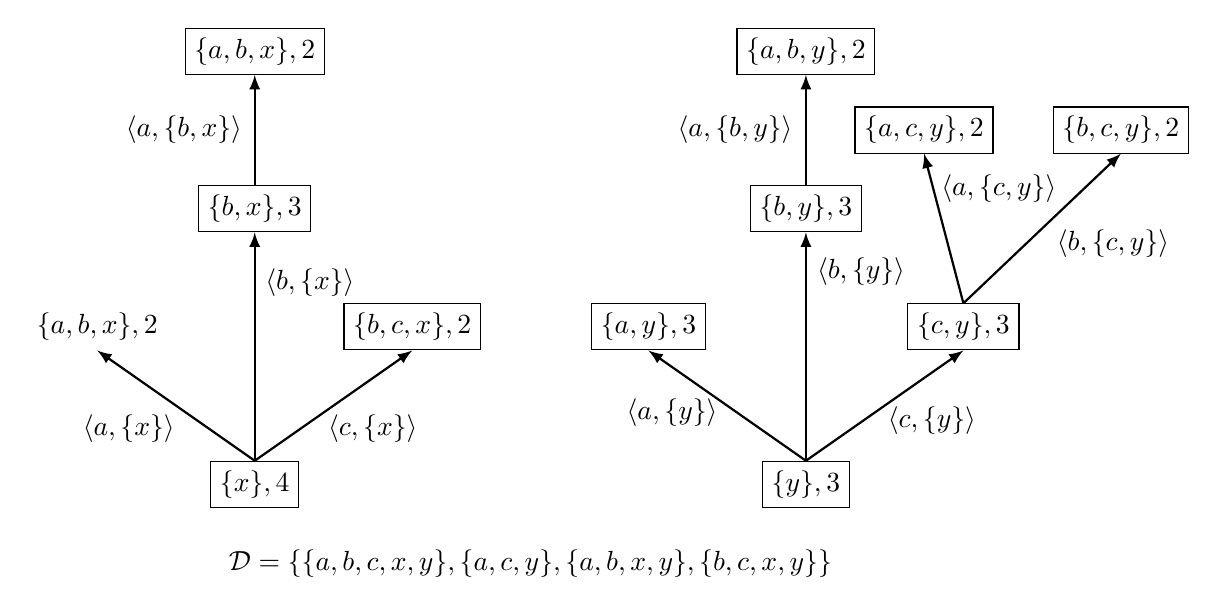
\begin{tikzpicture}[>=latex]%[>=triangle 45]
		\node(table) at (0,-1) {${\cal D}=\{\{a,b,c,x,y\}, \{a,c,y\}, \{a,b,x,y\}, \{b,c,x,y\}\}$};

		\node (x) [draw] at (-3.5,0) {$\{x\},4$};
		\node (y) [draw] at (3.5,0) {$\{y\},3$};
		\node (ax)  at (-5.5,2) {$\{a,b,x\},2$};
		\node (bx)  [draw] at (-3.5,3.5) {$\{b,x\},3$};
		\node (abx)  [draw] at (-3.5,5.5) {$\{a,b,x\},2$};
		\node (cx)  [draw] at (-1.5,2) {$\{b,c,x\},2$};
		\node (ay)  [draw] at (1.5,2) {$\{a,y\},3$};
		\node (by)  [draw] at (3.5,3.5) {$\{b,y\},3$};
		\node (aby)  [draw] at (3.5,5.5) {$\{a,b,y\},2$};
		\node (cy)  [draw] at (5.5,2) {$\{c,y\},3$};
		\node (acy)  [draw] at (5,4.5) {$\{a,c,y\},2$};
		\node (bcy)  [draw] at (7.5,4.5) {$\{b,c,y\},2$};
		\draw [->,thick] (x.north)--(ax.south) node[above, midway, xshift=-0.6cm, yshift=-0.6cm] {$\langle a, \{x\}\rangle$};
		\draw [->,thick] (x.north)--(bx.south) node[above, midway, xshift=0.7cm, yshift=0.5cm] {$\langle b, \{x\}\rangle$};
		\draw [->,thick] (x.north)--(cx.south) node[above, midway, xshift=0.5cm, yshift=-0.6cm] {$\langle c, \{x\}\rangle$};
		\draw [->,thick] (bx.north)--(abx.south) node[above, midway, xshift=-0.9cm, yshift=-0.3cm] {$\langle a, \{b,x\}\rangle$};
		\draw [->,thick] (y.north)--(ay.south) node[above, midway, xshift=-0.7cm, yshift=-0.4cm] {$\langle a, \{y\}\rangle$};
		\draw [->,thick] (y.north)--(by.south) node[above, xshift=0.7cm, yshift=-0.8cm] {$\langle b, \{y\}\rangle$};
		\draw [->,thick] (by.north)--(aby.south) node[above, midway, xshift=-0.9cm, yshift=-0.3cm] {$\langle a, \{b,y\}\rangle$};
		\draw [->,thick] (y.north)--(cy.south) node[above, midway, xshift=0.6cm, yshift=-0.5cm] {$\langle c, \{y\}\rangle$};
		\draw [->,thick] (cy.north)--(acy.south) node[above, midway, xshift=0.7cm, yshift=0.2cm] {$\langle a, \{c,y\}\rangle$};
		\draw [->,thick] (cy.north)--(bcy.south) node[above, midway, xshift=0.9cm, yshift=-0.5cm] {$\langle b, \{c,y\}\rangle$};
	\end{tikzpicture}

  \caption{\label{fig:capa:tree}
		\jlcm enumeration trees over an example dataset ${\cal D}$, with $\varepsilon=2$,
		in the \demoassoc case. Hence items in ${\cal B} = \{x,y\}$ are the only ones allowed as rules' consequent.
		An edge $\langle i, I \rangle$ represents an recursive invocation of \jlcm$(I, i)$.
		Only boxed nodes (closed itemsets satisfying the first-parent test) are returned.
		}
\end{figure}


Figure~\ref{fig:capa:tree} gives an example of the resulting enumeration.
It illustrates that Algorithm~\ref{alg:capa:lcm} allows \capa to obtain itemsets
that can be converted to the desired association rules $A \rightarrow {b}$.
It also computes $\mathit{support}({b})$ and $\mathit{support}(A \cup {b})$,
but we still need $\mathit{support}(A)$,
Thus, while CIS are outputted by \jlcm we also materialize the set of all antecedent
itemsets whose support needs to be evaluated as a prefix tree.
In a post-processing step, we read $\cal D$ once to compute their support.
This two-step approach avoids the computation of many itemsets that never appear as a rule antecedent.






\subsection{Exploitation step: ranking and displaying associations}
\label{sec:capa:exploit}

The last step in \capa is to show ranked lists of association rules to the analyst.
She should be able to switch easily from a ranking to another,
hence we pre-compute all rankings just after the mining step.

The quality measures we selected require $P(A)$, $P(B)$ and $P(A \cup B)$. % because,
%given $|{\cal D}|$, other probabilities like $P(B|A)$ or $P(A \neg B)$ can be derived from them.
We denormalize the results of the mining phase in order to store these 3 probabilities along each $A$ and $B$.
Thus each row represents an association rule and has enough information to compute its score.
This table is then augmented with \nbm columns,
one for each measure implemented. % in \capa, and listed in Table~\ref{tab:measures}.
The complete table is stored in a relational database
in order to ease the exploration by the final application.

The final component of \capa is a Web application allowing the analyst to explore this augmented table.
In any scenario (\demoassoc, \prodassocreceipt or \prodassocclient),
the analyst picks a measure and selects a target product or category, or a set of target products or categories.
This selection is made by navigating the product taxonomy in a top-down fashion.
Finally, association rules are returned in a table and sorted according to the selected measure,
as shown in Figure~\ref{fig:capa:screenshot}.

A rule like $\mathit{yogurt}\rightarrow\mathit{cheese}$ is displayed with 3 values:
\emph{support} (number of customers who bought both cheese and yogurt),
\emph{confidence} (fraction of yogurt buyers who also bought cheese)
and \emph{recall} (fraction of cheese buyers who also bought yogurt).
During the user study these figures help the analyst to quickly judge the volume of sales of each association.

To simplify the analysts' work in our user study (Section~\ref{sec:xp:user}),
the application does not propose \nbm measures.
Instead it proposes only 5 measures,
each one representative of each measures group identified by our quantitative study.

\begin{figure}
  \centering
  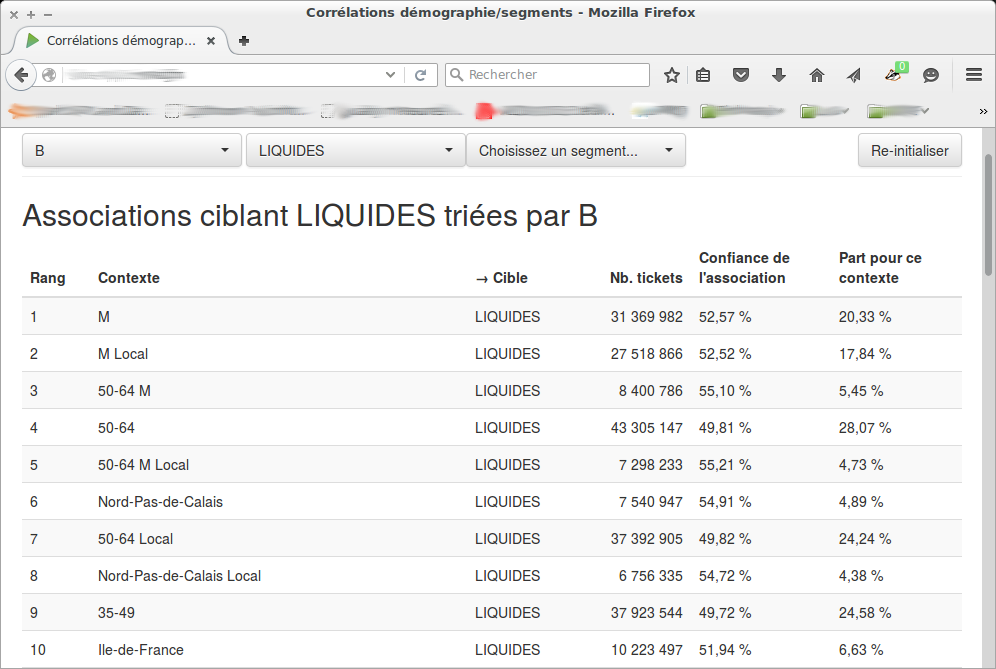
\includegraphics[width=\textwidth]{fig/screenshot_exploration.png}
  \caption{\label{fig:capa:screenshot}Screenshot of the exploration application presented to analysts.}
\end{figure}








\section{Quantitative study}
\label{sec:xp:empirical}

%We present an empirical evaluation of the \nbm measures for association rules introduced in the previous section.
The goal of the following evaluation is to automatically detect similarities between
interestingness measures and reduce the number of candidate measures to present to analysts in the user study of Section~\ref{sec:xp:user}.
To this end, we generate association rules for our 3 mining scenarios
and evaluate the pairwise similarity of the \nbm rankings produced by the measures we selected.
%In order to assist the analyst in selecting measures,
%the following evaluation consists in comparing rankings produced by these measures on our data,
%to discover which measures differ significantly in practice.
We then use these similarities to classify ranking measures into \emph{groups},
and annotate these groups based on common properties.
%We discuss key insights obtained from rigorous experimentation on each group.

We first present in Section~\ref{sec:correlations} the similarity measures used to compare our ranked lists.
These include a new one,
Normalized Discounted Correlation Coefficient ({\em NDCC}),
whose score is more influenced by top results.
Then, we compare quality measures in two different cases:
rules having the same target (Section~\ref{sec:identicaltargets}) and rules having different targets (Section~\ref{sec:differenttargets}).
We conclude this evaluation with the selection of representative measures in Section~\ref{sec:selection}.

\subsection{Ranking similarity measures}
\label{sec:correlations}

We use four methods to compare the ranked lists obtained in our 3 mining scenarios.
The first three methods are taken from the literature.
We then introduce {\em NDCC}, a new parameter-free ranking similarity designed to emphasize differences at the top of the ranking.

In the following $\mf R$ denotes the set of association rules obtained from the mining phase.
We interpret each quality measure $m$ as a function that receives a rule and generates a score,
$m:{\mf R}\rightarrow \mathbb{R}$.
We use $L_{\mf R}^m$ to denote the ordered list of rules in $\mf R$ sorted by decreasing score according to $m$.
Thus, $L_{\mf R}^m=<r_{1},r_{2},\ldots>$ s.t. $\forall i>i'\ m(r_{i})<m(r_{i'})$.
The rank of a rule $r$ in $L_{\mf R}^m$ is denoted $r^m$.
We generate \nbm lists, one for each measure $m$, from the same set of rules $\mf R$.
%$L_{\mf R}^m$ denotes a ranked list of association rules according to measure $m$
%where the rank of rule $r$ is given as $rank(r,L_{\mf R}^m)=|\{r'|r'\in \mf R,\ m(r')\geq m(r)\}|$.
To assess the dissimilarity between two measures $m$ and $m'$,
we compute the dissimilarity between their ranked lists, $L_{\mf R}^m$ and $L_{\mf R}^{m'}$.
%We use $r^m$ as a shorthand notation for $rank(r,L_{\mf R}^m)$.



\subsubsection{Spearman's rank correlation coefficient}

Given two ranked lists $L_{\mf R}^m$ and $L_{\mf R}^{m'}$,
{\em Spearman's rank correlation}~\cite{Daniel1978}
computes a linear correlation coefficient that varies between $1$ (identical lists)
and $-1$ (opposite rankings), as shown below.
$$\mathit{Spearman(L_{\mf R}^m,L_{\mf R}^{m'})} = 1 - \frac{6\sum\limits_{r\in \mf R}{(r^m-r^{m'})^2}}{|\mf R|(|\mf R|^2-1)}$$
This coefficient depends only on the difference between each rule's rank in the two lists,
and not on the ranks themselves.
Hence the penalization is the same for differences occurring at the beginning or at the end of the lists.


\subsubsection{Kendall's $\tau$ rank correlation coefficient}

{\em Kendall's $\tau$ rank correlation coefficient}~\cite{KendallBIOMETRIKA38}
is based on the idea of agreement among element (rule) pairs.
A rule pair is said to be \emph{concordant} if their order is the same in
$L_{\mf R}^m$ and $L_{\mf R}^{m'}$, and \emph{discordant} otherwise.
$\tau$ computes the difference between the number of concordant and discordant pairs and divides by the total number of pairs as shown below.

\begin{align*}
  \tau(L_{\mf R}^m,L_{\mf R}^{m'}) = & \frac{|C|-|D|}{\frac{1}{2}|\mf R|(|\mf R|-1)}  \text{, where: }\\
      C=\{(r_i,r_j)|& r_i,r_j\in \mf R\wedge i<j\wedge \\
                 &\sign({r_i^m-r_j^m}) = \sign(r_i^{m'}-r_j^{m'})\} \\
      D=\{(r_i,r_j)|& r_i,r_j\in \mf R\wedge i<j\wedge \\
                 &\sign({r_i^m-r_j^m}) \neq \sign(r_i^{m'}-r_j^{m'})\}
\end{align*}

As {\em Spearman}, $\tau$ varies between $1$ and $-1$ and penalizes uniformly across all ranks.


\subsubsection{Overlap@$k$}

Overlap@$k$ is a ranked lists  similarity measure widely used in Information Retrieval.
It is based on the premise that, in large ranked lists,
the analyst is only expected to look at the top few results, that are highly ranked.
While {\em Spearman} and $\tau$ account for all elements uniformly,
Overlap@$k$ compares two rankings by computing the overlap between their top-$k$ elements only.
We use $k \in \{10, 20, 50, 100, 500, 1000\}$.

$$\mathit{Overlap@k(L_{\mf R}^m,L_{\mf R}^{m'})=\frac{|\{r\in \mf R| r^m\leq k\}\cap\{r\in \mf R|r^{m'}\leq k\}|}{k}}$$


\subsubsection{Normalized Discounted Correlation Coefficient}
%\label{sec:ndcc}
Overlap@$k$, {\em Spearman} and $\tau$ sit at two different extremes.
The first takes only into account the top $k$ elements of each list,
whereas the latter two consider all parts of the lists uniformly.
In our use case, we aim for a good trade-off between these extremes.

To bridge this gap, we propose a new ranking correlation measure coined
\emph{Normalized Discounted Correlation Coefficient} or {\em NDCC}.
{\em NDCC} draws inspiration from {\em NDCG, Normalized Discounted Cumulative Gain}~\cite{JarvelinACM02},
a ranking measure commonly used in Information Retrieval.
The core idea in {\em NDCG} is to reward a ranked list $L_{\mf R}^m$ for placing an element $r$
of relevance $\mathit{rel_r}$ by $\frac{\mathit{rel_r}}{\log{r^m}}$.

The logarithmic part acts as a smoothing discount rate representing the fact that as the rank increases,
the analyst is less likely to observe $r$.
In our setting there is no ground truth to properly assess $\mathit{rel_r}$.
Instead, we use the ranking assigned by $m'$ as a relevance measure for $r$,
with an identical logarithmic discount.
When summing over all of $\mf R$, we obtain $\mathit{DCC}$,
which presents the advantage of being a symmetric correlation measure between two rankings $L_{\mf R}^m$ and $L_{\mf R}^{m'}$.
$$\mathit{DCC(L_{\mf R}^m,L_{\mf R}^{m'})}=\sum_{r\in \mf R}{\frac{1}{\log{(1+r^{m'})}\log{(1+r^m)}}}$$
We compute $\mathit{NDCC}$ by normalizing $\mathit{DCC}$ between
$1$ (identical rankings) and $-1$ (reversed rankings).

\begin{equation*}
\begin{split}
    \mathit{NDCC(L_{\mf R}^m,L_{\mf R}^{m'})}&=\frac{dcc-avg}{max-avg}\\
\mbox{where } dcc&=\mathit{DCC(L_{\mf R}^m,L_{\mf R}^{m'})}\\
    max&=\mathit{DCC(L_{\mf R}^{m'},L_{\mf R}^{m'})}\\
    min&=\mathit{DCC(L*,L_{\mf R}^{m'})},\ L*=\mathit{rev(L_{\mf R}^{m'})}\\
    avg&=(max+min)/2
\end{split}
\end{equation*}



\pagebreak



\subsubsection{Ranking comparison by example}

We illustrate the difference between all ranking correlation measures with an example in Table~\ref{tab:exampleranks}.
This shows correlation of a ranking $L^1$ with 3 others, according to each measure.
$\mathit{NDCC}$ does indeed penalize differences at higher ranks, and is less sensitive at lower ranks.

\begin{table}
  \begin{center}
    \begin{tabular}{c|c}
      Ranking & Content\\
      \hline
      $L^1$& $r_1,r_2,r_3,r_4$ \\
      $L^2$& $r_2,r_1,r_3,r_4$ \\
      $L^3$& $r_1,r_2,r_4,r_3$  \\
      $L^4$& $r_2,r_3,r_1,r_4$ \\
    \end{tabular}
    \begin{tabular}{c|c|c|c|c}
      &$\mathit{Spearman}$&$\tau$&$\mathit{Overlap}$@$2$&$\mathit{NDCC}$\\
      \hline
      $L^2$&$0.80$&$0.67$&$1$&$0.20$\\
      $L^3$&$0.80$&$0.67$&$1$&$0.97$\\
      $L^4$&$0.40$&$0.33$&$0.5$&$-0.18$\\
    \end{tabular}
    \caption{Example rankings,
      and correlations between $L^1$ and the three other rankings.
    \label{tab:exampleranks}}
  \end{center}
\end{table}




\subsection{Ranking rules with identical targets}
\label{sec:identicaltargets}
We first consider the case of ranking association rules $A\rightarrow B$ where $B$ is a single product or category,
{\em i.e.} all rules have the same $B=\{b\}$.
We perform a comparative analysis of ranking measures on our 3 mining scenarios,
which lead to similar conclusions.
We use as targets for this comparison 64 products or categories previously studied by analysts.
We compute one rule ranking per interestingness measure.

While all measures are computed differently,
we notice that some of them always return the  same ranking for association rules of a given target.
We identify them in Table~\ref{tab:measures} (p.\pageref{tab:measures}) using symbols.
We also observe important similarities.
For example, in \prodassocclient,
the 64 targets provide \num{1651024} association rules.
89\% of rankings are equal with {\em Sebag-Schoenauer} and {\em lift},
or 87\% with {\em Loevinger} and {\em lift}.
This difference between the number of interestingness measures considered (39)
and the number of different rankings obtained (31)
can easily be explained analytically in the case of a fixed target.
Indeed, for a given ranking, $P(B)$ is constant,
which eliminates some of the differences between interestingness measures.
In addition, some measures only have subtle differences which only appear when selecting extreme values
for $P(A)$, $P(B)$ and $P(AB)$, which do not occur in practice in our retail datasets.

\subsubsection{Comparative analysis}
We now evaluate similarity between interestingness measures that do not return the same rankings.
We compute a \nbm$\times$ \nbm correlation matrix of all rankings according to each correlation measure described in Section~\ref{sec:correlations},
and average them over the 64 target products.
This gives us a ranking similarity between all pairs of measures.
We then rely on hierarchical clustering with average linkage~\cite{sokal58}
to obtain a dendrogram of interestingness measures and analyze their similarities.
Figure~\ref{fig:capa:dendogram:identical} shows the clustering by {\em NDCC}
in the \demoassoc scenario;
the dendrograms for $\mathit{NDCC}$ and $\tau$ in our three scenarios are presented in
Annex~\ref{sec:capa:clusters:identicaltargets}, p.\pageref{sec:capa:clusters:identicaltargets}.
For better readability, we merge sub-trees when correlation is above $0.9$.
To describe the results more easily, we partition interestingness measures into 5 groups,
as indicated in the third column in Table~\ref{tab:measures}.


\begin{figure}[th!]
  \begin{center}
  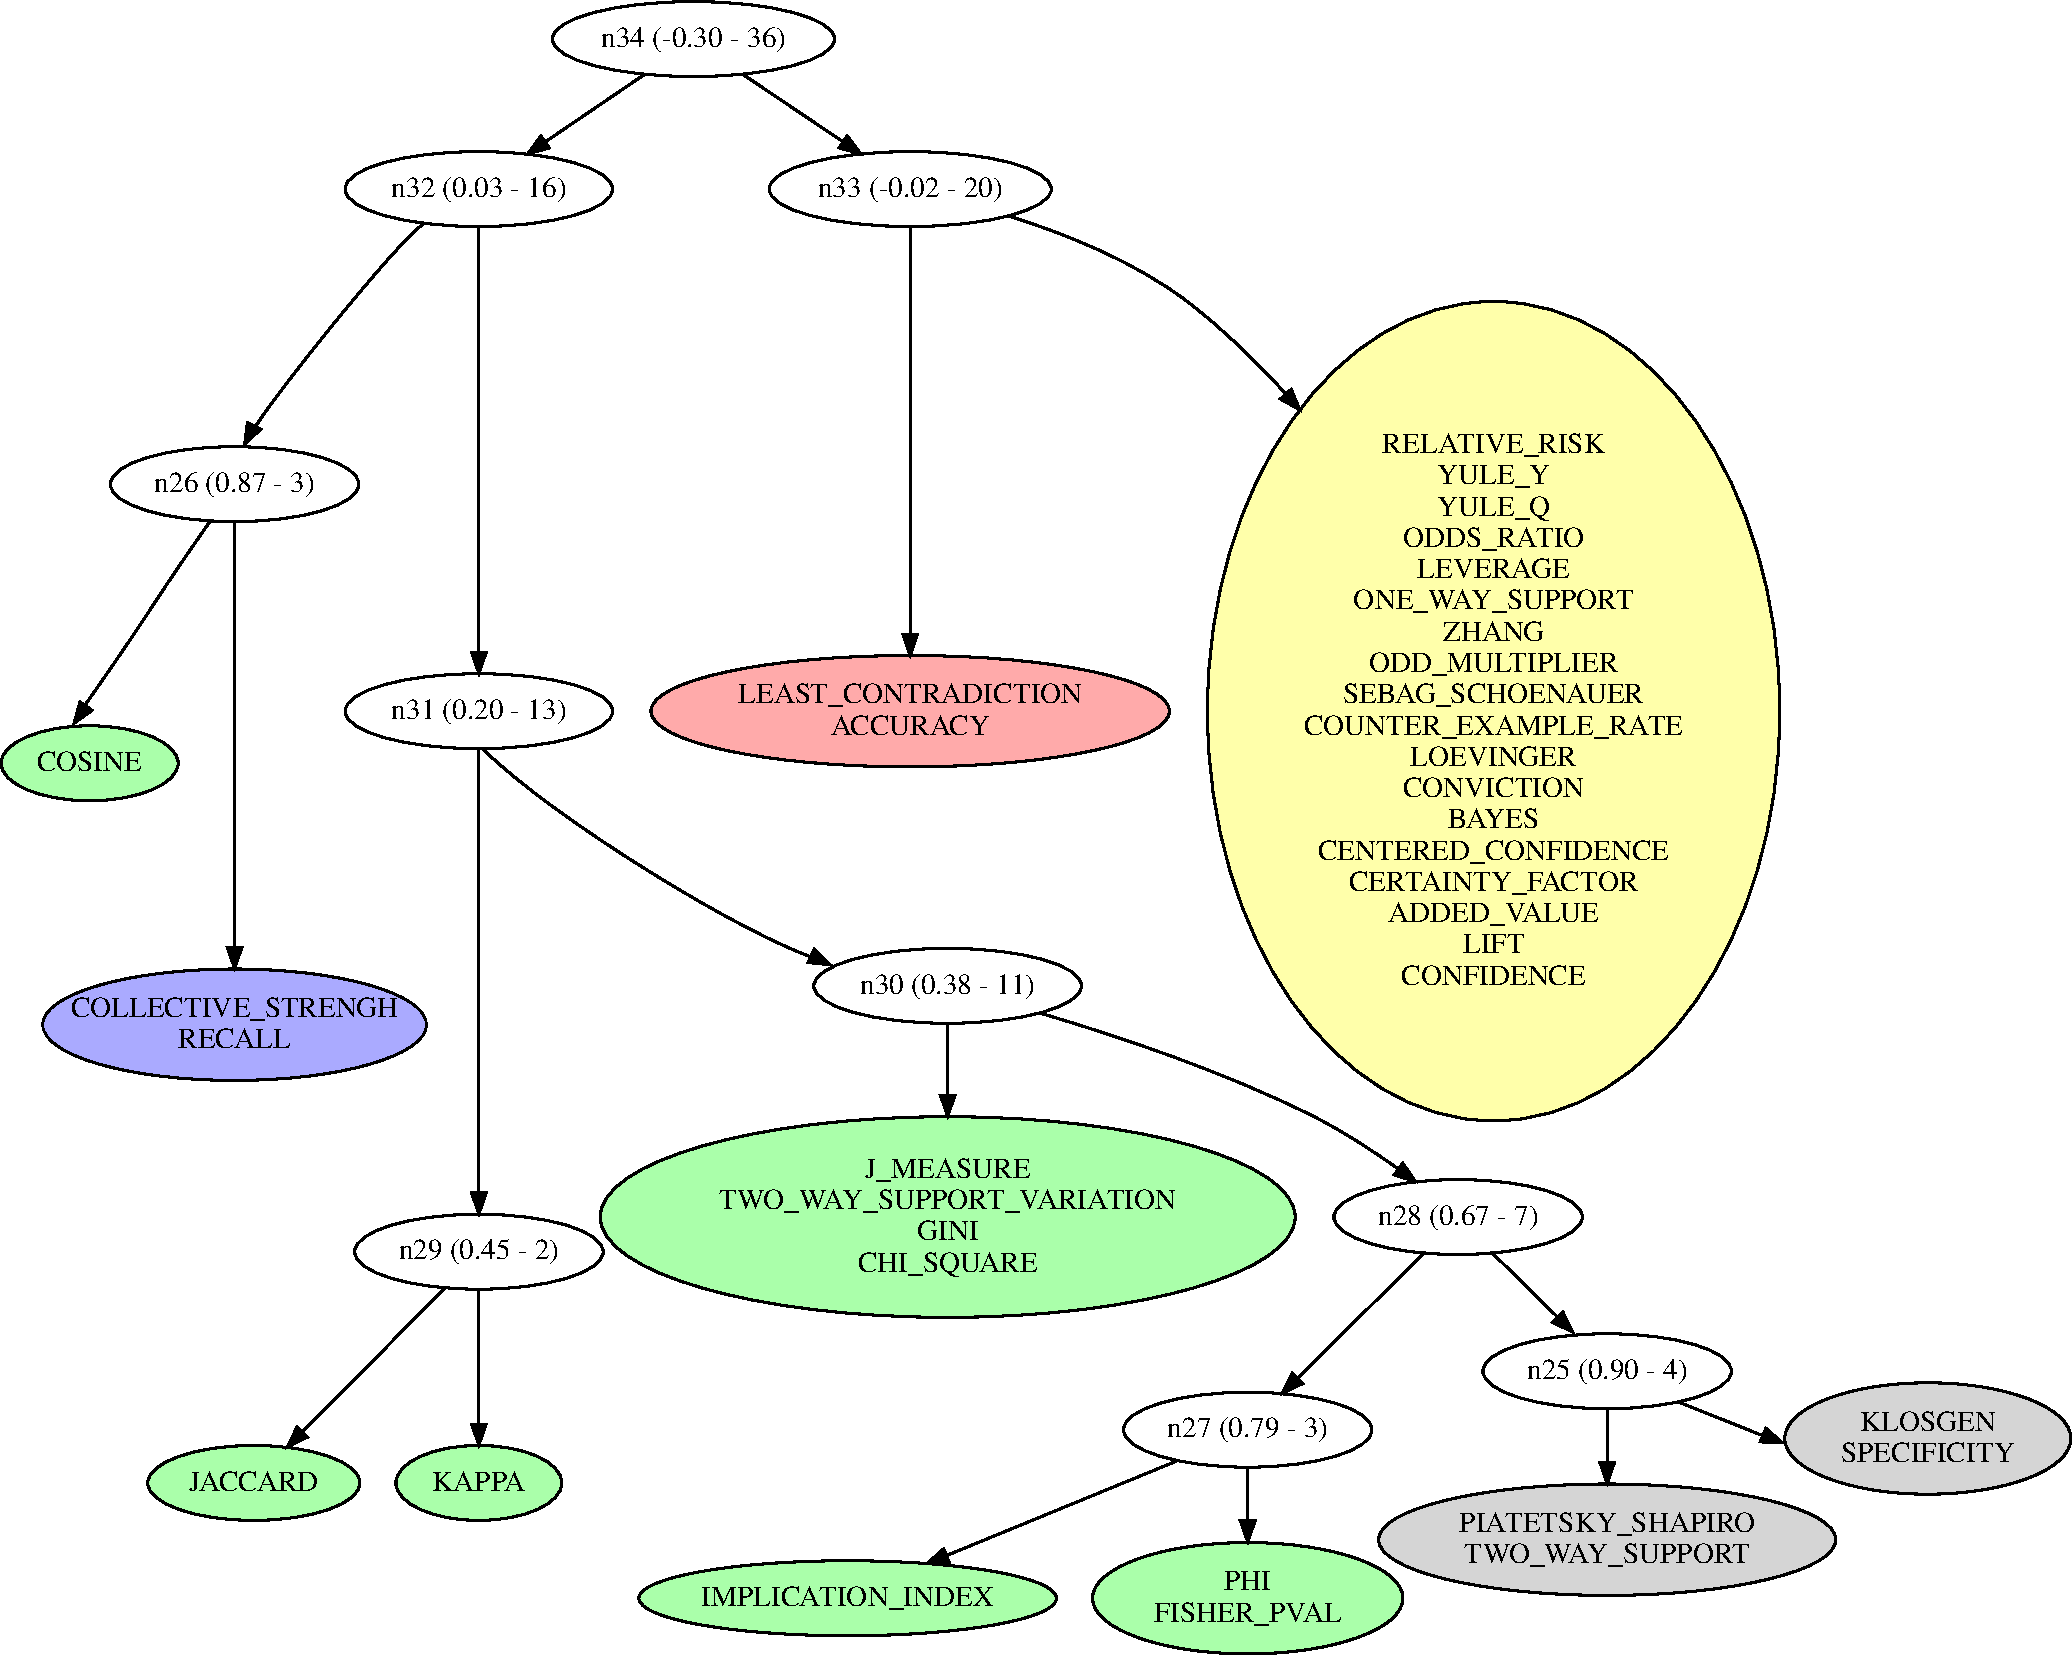
\includegraphics[width=\textwidth]{svg/rankingcom/patterns_demo-perTarget-NDCG.pdf}
  \caption{Clustering of quality measures,
    by {\em NDCC} in the \demoassoc scenario for association rules having identical targets.
    \label{fig:capa:dendogram:identical}}
  \end{center}
\end{figure}


$G_1$ is by far the largest group: in addition to 4 measures that always generate the same rankings,
14 other measures output very similar results.
A second group, $G_2$, comprising 2 measures, is quite similar to $G_1$ according to $\mathit{NDCC}$,
especially for \prodassocclient.
$\tau$ also discovers this similarity, but considers it lower,
which shows that it is mostly caused by high ranks.
The most dissimilar group is $G_5$.
We note that $G_1$, $G_2$ and $G_5$ are extremely consistent across our 3 scenarios.
The two other groups, $G_3$ and $G_4$,
each have a constant ``core'' of measures.
But {\em Klosgen}, {\em Jaccard}, {\em Two-way support} and {\em Cosine} are not
always clustered with the same group.
Their rankings differ more or less at each extreme of the lists.
%Indeed, when focusing on the first 20 elements ($\mathit{Overlap}$@$20$),
%only an average of 71\% are shared between {\em Jaccard} and the rest of $G_3$.

% This situation also occurs between {\em Klosgen} and the rest of $G_5$.
% Interestingly, we observe that, according to $\mathit{NDCC}$,
% $G_4$ is closest to $G_5$ and is negatively correlated with the other groups.
% However, according to $\tau$, $G_4$ is very similar to $G_3$ and is negatively correlated with $G_5$.
%
% This difference of behavior between ranking measures illustrates the importance of accounting for rank positions.
% When the top of the ranking is considered more important, some similarities emerge.





\pagebreak

\begin{figure}[th!]
  \begin{center}
  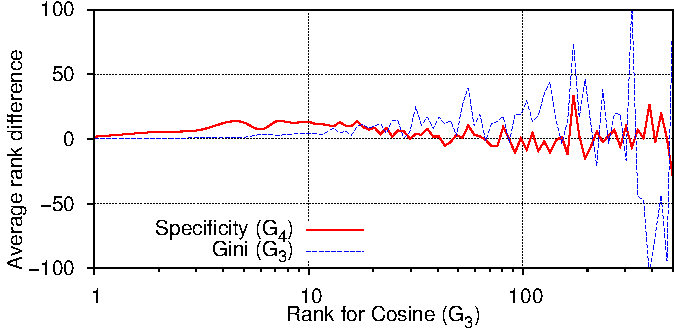
\includegraphics{fig/capa/rank-correlation.pdf}
  \caption{Rank differences between {\em Cosine} and {\em Specificity},
    and {\em Cosine} and {\em Gini}.
    \label{fig:rankcorrelation}}
  \end{center}
\end{figure}

We illustrate this behavior in Figure~\ref{fig:rankcorrelation}
by displaying correlation between rankings obtained with different interestingness measures.
This experiment clearly shows that overall, {\em cosine} ($G_3$) is closer to {\em specificity}
($G_4$) than {\em Gini} ($G_3$), as the observed rank difference is overall smaller.
However, when focusing on the top-10 results of {\em cosine},
{\em Gini} assigns closer ranks than {\em specificity}.
This explains the difference in clustering between $\mathit{NDCC}$ and $\tau$,
and motivates our choice to assign such outlier measures to $G_3$ or $G_4$.
Our group assignment for these measures also takes into account clusterings according to
$\mathit{Spearman}$ and $\mathit{overlap}@50$.

\subsubsection{Annotating groups}
\label{sec:annotation}

\begin{figure}
  \centering
  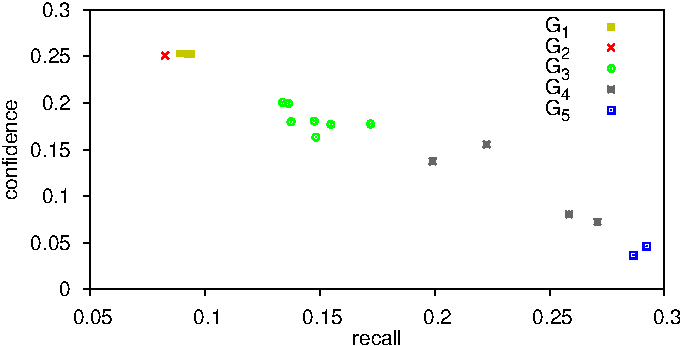
\includegraphics{fig/capa/recall_precision}
  \caption{Average recall/confidence of the top-20 results of interestingness measures
    \label{fig:recallprecision}
  }
\end{figure}

While using hierarchical clustering on interestingness measures allows the discovery of groups of measures
and their relative similarity, it does not fully explain which types of results are favored by each of them.
We propose to compare their outputs according to the two most basic and intuitive interestingness measures employed in data mining:
{\em recall} and {\em confidence}.
{\em recall} represents the proportion of target items that can be retrieved by a rule, that is,  $P(A|B)$.
Its counterpart, {\em confidence}, represents how often the consequent is present when the antecedent is, that is, $P(B|A)$.
We present, in Figure~\ref{fig:recallprecision}, the average {\em recall} and {\em confidence}
of the top-20 rules ranked according to each interestingness measure.
$G_1$ contains {\em confidence}, so it is expected to score the highest on this dimension.
$G_2$ is extremely close to $G_1$, but obtains slightly lower {\em confidence} and {\em recall}.
We then have, in order of increasing {\em recall} and decreasing {\em confidence} $G_3$ and $G_4$.
Finally, $G_5$, which contains {\em recall}, obtains the highest {\em recall} but the lowest {\em confidence}.
Figure~\ref{fig:recallprecision} also shows that executing a Euclidean distance-based clustering,
 such as $k$-means, with recall/confidence coordinates would lead to groups similar to the ones obtained with hierarchical clustering.
Hence, this analysis is consistent with the hierarchical grouping and the correlation with $\mathit{NDCC}$.

While we believe that $\mathit{NDCC}$ reflects better the interpretation of analysts browsing rules,
it is important to note that the grouping of interestingness measures created through this evaluation
is stable across all 4 correlation measures and for all 3 scenarios.
Correlation between different groups of measures may vary, but measures within a single group always have a high similarity.
Thus, we state that the obtained results are true in the general case of food retailers
and we can rely on these groups to reduce the number of options presented to analysts.



\subsection{Ranking rules with  different targets}
\label{sec:differenttargets}
We now consider the problem of ranking association rules when many targets are provided as input,
i.e. association rules $A \rightarrow B$ can have different targets $b \in {\cal B}$.
Compared to having a single target,
this setting introduces one more degree of freedom in the quality measure of the association rules,
as $P(B)$ varies.
We rely on the same set of (64) products as in the identical target experiment,
but instead of generating rankings for each target, we rank all association rules together.
The dendrograms of quality measures obtained for $\mathit{NDCC}$ and $\tau$ are presented in
Annex~\ref{sec:capa:clusters:differenttargets}, p.\pageref{sec:capa:clusters:differenttargets}.
Only Yule's Q, Yule's Y and Odds Ratio produced identical rankings.

We observe a much wider variety in rankings, which is expected given the presence of one more parameter.
The group $G_1$, observed previously, splits into two different sub-groups, $G_1^a$ and $G_1^b$.
A large fraction of $G_3$ remains similar,
but the two measures that constitute $G_2$ and $G_5$ are not correlated in all scenarios.
$G_2$ and $G_4$ are not preserved when ranking different targets simultaneously.
We observe a stronger agreement between $\mathit{NDCC}$ and $\tau$.
% The only notable differences are \textit{(i)}
% {\em Klosgen} and {\em Gini}, which are highly correlated with $G_4$ when focusing on the top results,
% while they are more similar to $G_1^a$ globally,
% and \textit{(ii) Jaccard},
% which switches from a similarity with {\em Piatetsky-Shapiro} to a similarity with $G_6$.

Measures that prioritize high values of $P(B)$,
i.e. favor targets that are more frequent, are $G_1^a$, {\em Piatetsky-Shapiro}, {\em Klosgen} and {\em Gini}.
Indeed, in the case of {\em confidence} ($G_1^a$),
an association rule $A\rightarrow B$ that has a very frequent $B$
can easily score highly by selecting a very specific $A$.
Conversely, {\em specificity}, {\em collective strength}, {\em accuracy}, {\em recall} and
measures of $G_1^b$ tend to rank less frequent targets highly.
A similar explanation applies to {\em recall},
as a low frequency of $B$ makes it easier to find association rules that capture most of its appearances in the data.



\subsection{Selecting representative measures}
\label{sec:selection}
We summarize the findings of the comparative evaluation in Table~\ref{tab:groupsummary}.
When the analyst selects a single target, we identify 5 groups of measures that behave similarly.
When multiple targets are selected, $G_1$ splits into 2 sub-groups.
Each group offers a different trade-off in terms of confidence and recall, and thus ranks association rules differently.
When ranking rules with different targets, some groups are sensitive to the frequency of the target.

We select the quality measure that most represents each group of measures (i.e. with highest average similarity)
in order to confront the results of this analysis with the opinion of domain experts in our user study.
Taking a general data mining perspective leads us to considering $G_3$ and $G_4$
as the most promising groups for finding interesting association rules.
Indeed, it is important to achieve a good trade-off between {\em recall} and {\em confidence}
in order to find reliable association rules that can be applied in a significant number of cases.
For example the {\em F1} score, that combines {\em recall} and {\em confidence}, would prefer $G_3$ and $G_4$ to others.
The goal of our user study is to confront this intuition to marketing experts' opinion.

\begin{table}[tb]
\centering
\begin{tabular}{|l|l|}
\hline
\begin{tabular}{l}Group\\Representative\end{tabular}&Description\\\hline
\cellcolor{g1aColor}\begin{tabular}{l}$G_1^a$\\Lift\end{tabular}&\begin{tabular}{l}Highest precision\\Very low recall\\Favors frequent targets\end{tabular}\\\hline
\cellcolor{g1bColor}\begin{tabular}{l}$G_1^b$\\Added value\end{tabular}&\begin{tabular}{l}Highest precision\\Very low recall\\Favors rare targets\end{tabular}\\\hline
\cellcolor{g2Color}\begin{tabular}{l}$G_2$\\Accuracy\end{tabular}&\begin{tabular}{l}Very high precision\\Very low recall\end{tabular}\\\hline
\cellcolor{g3Color}\begin{tabular}{l}$G_3$\\Fisher's exact test\end{tabular}&\begin{tabular}{l}High precision\\Low recall\\Low sensitivity to target frequency\end{tabular}\\\hline
\cellcolor{g4Color}\begin{tabular}{l}$G_4$\\Piatetsky-Shapiro\end{tabular}&\begin{tabular}{l}Low precision\\High recall\end{tabular}\\\hline
\cellcolor{g5Color}\begin{tabular}{l}$G_5$\\Collective strength\end{tabular}&\begin{tabular}{l}Lowest precision\\Highest recall\\Favors rare targets\end{tabular}\\\hline
\end{tabular}
\caption{Summary of quality measure groups\label{tab:groupsummary}}
\end{table}










\vfill
\pagebreak


\section{User study}
\label{sec:xp:user}

We now report the results of a user study with domain experts from Intermarch\'e.
The goal of this study is to assess the ability of interestingness measures to rank association rules
according to the needs of an analyst.
In the previous section we identified 5 groups of measures,
and selected a representative of each group for the user study (Table~\ref{tab:groupsummary}).
We rely on the expertise of our industrial partner to determine, for each analysis scenario,
which group produces the most interesting results.
This experiment involved 2 experienced analysts from the marketing department of Intermarch\'e.
%We setup \capa and let analysts select targets multiple times in order to populate
%the web application's database with association rules.
We let them interact with \capa without any time restriction,
and collect their feedback in a free text form.

Each analyst firstly has to pick a mining scenario among \demoassoc, \prodassocreceipt, or \prodassocclient.
Then she picks a target category or a target product in the taxonomy.
In \prodassocreceipt\ and \prodassocclient, she also has the option to
filter out rules whose antecedent products are not from the same category as the target.
Finally, she chooses one of our 5 ranking measures to sort association rules.
Neither the name of the measure nor its computed values for association rules are revealed,
because we wanted analysts to evaluate rankings without knowing how they were produced.
Resulting association rules are ranked according to a selected measure.
Each rule is displayed with its support, confidence and recall,
such that analysts can evaluate it at a glance
(see Figure~\ref{fig:capa:screenshot}, p.\pageref{fig:capa:screenshot}).
For each scenario,
our analysts are asked which representative measure highlights the most interesting results.
As detailed below, in all cases a few of them were chosen.
%They also answered the following questions:
%{\em What is your first impression?
%How many rules are interesting?
%Do those rules overlap with your experience or former studies?}

\subsection{Scrolling behavior}
Once the analyst selects a target, \emph{all} matching rules are returned.
The initial motivation of this choice was to determine how many results
are worth displaying and are actually examined by the analysts.
According to the follow-up interview with the analysts, they carefully considered the first ten results,
and screened up to a hundred more.
Interestingly, analysts mentioned that
they also scrolled down to the bottom of the list
in order to see which customer segments are not akin to buying the selected category.
For example, when browsing demographic association rules,
they expected to find \{{\em 50-64}\} $\rightarrow$ {\em pet food} among top results,
but also expected \{{\em <35, Paris}\} $\rightarrow$ {\em pet food} among bottom results.
This confirms that all rules should remain accessible.
This also indicates that while interestingness measures favor strong associations,
it would also be interesting to highlight {\em anti}-rules, as those can also convey useful information.

\subsection{Feedback on ranking measures}
We let marketing experts explore all 3 scenarios and express their preference towards groups of measures.

In the \demoassoc case, $G_1$ and $G_3$ were both highly appreciated.
$G_1$ favors rules such as $\{< 35, M, $ Oise$\}\rightarrow$ {\em Flat and Carbonated drinks}.
These rules are very specific and thus have a very high confidence (31,58 \% in this particular case).
However, this comes at the cost of recall (0,08 \%).
Experts value {\em confidence} much more than {\em recall}, as their priority is finding rules that they consider reliable.
A low support is not necessarily an issue, and can lead to the discovery of surprising niche rules that can be exploited nonetheless.
As discussed in Section~\ref{sec:annotation},
$G_3$ offers a more balanced trade-off between confidence and recall,
and prioritizes rules such as $\{$< 35, *, *$\}\rightarrow$ {\em Baby food} (confidence 8,57 \%, recall 37,61\%).
These rules are interesting because they capture a large fraction of the sales of a given category, but are less reliable and generally less surprising.
$G_2$ and $G_4$ were considered as less interesting than $G_1$ and $G_3$ respectively.
Their results offer similar trade-offs, but with lower confidence each time.
$G_5$ was considered unusable because of its very low confidence.

When experimenting with \prodassocclient or \prodassocreceipt, we observed a slightly different behavior.
By default, the analysts favored $G_1$ and $G_2$ because of the confidence of their results.
Then, we offered the analysts the possibility of filtering the rules to only keep the ones in which the antecedent contains products from the same category as the target.
This led to analysts favoring $G_3$ and $G_4$.
This difference is caused by an important but implicit criterion: the ability of a measure to filter out very popular products.
For example, the rule \{{\em vanilla cream, emmental}\}$\rightarrow$ {\em chocolate cream}
usually appears just above its shorter version
\{{\em vanilla cream}\}$\rightarrow$ {\em chocolate cream},
because the first one has a confidence of $32\%$ and the second $31\%$.
However, experts prefer the second one,
because \textit{emmental} (cheese) is one of the star products we mentioned in Section~\ref{sec:toppi:stars}.
Hence its addition to the rule is considered insignificant.
This ``noise'' generally increases with {\em recall}.
Hence, when no filtering is available, $G_1$ is selected, but analysts prefer the {\em recall} and {\em confidence} trade-off provided by $G_3$ and $G_4$.
Again, $G_4$ suffered from its proximity to $G_3$ with lower confidence, while $G_5$'s confidence was too low.









\section{Conclusion}
\label{sec:capa:conc}

From a dataset of transactions,
created by our curation module according to one of our 3 mining scenarios,
\capa extracts association rules containing targets pre-selected by the analyst.
It then allows to compare how \nbm interestingness measures~\cite{GengACM06,Lenca2007} rank these associations.
%We presented quantitative and qualitative comparisons,
%from which we can infer practical advice to highlight high-quality associations in the food retail domain.
%Those are developed in Section~\ref{sec:capa:strat}.
Although the quality measures yield very different absolute values,
when ranking association rules many of them are similar, or even identical.

Our first comparison is quantitative:
we generate and rank association rules,
and compare the rankings obtained by the measures we selected.
We show that interestingness measures can be automatically grouped
into 5 groups of similar rankings, regardless of the mining scenario.
These groups are consistent across our 3 mining scenarios and 4 similarity measures.
Our choice of similarity measures include a novel one: Normalized Discounted Correlation Coefficient {\em{(NDCC)}}.
Our motivation to propose {\em NDCC} is to give more importance to top rules in the similarity evaluation.
Hence it fits our use case, where analysts are interested in the first few dozen associations.

Our second comparison is qualitative, and involves two experienced domain experts from Intermarch\'e.
The goal of this user study is to find which of the 5 groups of interestingness measures
are meaningful in the food retail domain.
Results suggest that no measure fits the general case:
their preference depends on whether the initial constraints are highly selective or not.
In all cases, analysts mentioned $G_5$ (see Table~\ref{tab:measures}, p.\pageref{tab:measures})
as uninteresting overall because it selects rules of low {\em confidence}.
Thus, sorting by decreasing {\em lift}
(which is close to sorting by decreasing {\em confidence})
is the most preferred choice.
Combined with the minimum support threshold used in the mining phase, this ranking promotes rules that are considered reliable.
However, the preference of the analysts changes when filters are available to narrow down the set of rules to specific product categories.
In this case, they favor the compromise between {\em confidence} and {\em support} offered,
for instance, by the {\em Piatetsky-Shapiro}'s measure~\cite{PiatetskyKDD91}.
That is because filtering allows them to get rid of noisy products.


To the best of our knowledge, \capa targets datasets which are orders of magnitude bigger (and sparser)
than those tested in existing work on ranking association rules.
The present work is also the first to complement a quantitative analysis
with a user study involving domain experts.
Therefore the groups of measures and recommendations we present here differ from the studies mentioned in
Section~\ref{sec:rel:capa} (p.\pageref{sec:rel:capa}).

The highest scoring measures in~\cite{LeSANER15} all belong to our groups
$G_1$ and $G_3$, which were also favored by our analysts.
But a few measures from our $G_1$ are scoring poorly in~\cite{LeSANER15},
hence our measures of choice do not match theirs, overall.
The largest group identified by \textsc{Herbs}~\cite{Lenca2007,VaillantDS04} is quite similar to $G_1$ and also includes {\em confidence}.
But there are also significant differences.
For instance, we find $G_2$ and $G_5$ to be very different,
while~\cite{Lenca2007} considers the measures of these two groups as similar.
The authors observe a weak resemblance between the theoretical and experimental analysis of the measures.
The main similarity between \textsc{Herbs} and
\capa is the reliance on a pairwise correlation measure followed by a hierarchical clustering to detect groups of measures.
But \capa is entirely focused on retail data,
which has different properties and contains millions of transactions and rules.
\capa is also more exhaustive in the analysis of measures:
we consider more interestingness measures, and 4 different ranking correlation measures, instead of Kendall's $\tau$ only.
%This allows us to discover more subtle differences in a more specific domain.
%Finally, we perform a user study to assess the quality of each group according to experts
%from the retail industry.
Such differences in the results highlight the importance of performing domain-specific studies,
as the properties of data and the expectations of analysts vary significantly.













Overall, the quality measures we selected with \capa allow the analyst to pick
a few dozen associations of great interest out of the thousands available.
We observe this in our 3 mining scenarios, both for highly-targeted analyzes
(when the analyst specifies a narrow set of target items)
and in an exploratory setting.
In the latter case, these quality measures can re-rank the item-centric itemsets lists produced by \toppi.
%During a more precise study, they can be used
This chapter therefore allows us to display interesting associations in all variants of the \datalyse project.



% Our study lets analysts choose one of 3 mining scenarios, along with target products or categories.
% Analysts also choose an interestingness measure without revealing its name.
% Their interactions with the resulting list of association rules were
% observed and their feedback recorded in a free-text form.
% Overall, ranking rules by decreasing confidence was mostly preferred.
% Combined with the minimum support threshold used in the mining phase,
% this ranking promotes rules that are considered reliable.
% However,
% the preference of the analysts changes when filters are available
% to narrow down the set of rules to specific product categories.
% In this case, they favor the compromise between confidence and support offered, for instance,
% by the Piatetsky-Shapiro's measure~\cite{PiatetskyKDD91}.
%
%
% Overall, ranking rules by decreasing confidence was mostly preferred.
% Combined with the minimum support threshold used in the mining phase,
% this ranking promotes rules that are considered reliable.
% However,
% the preference of the analysts changes when filters are available
% to narrow down the set of rules to specific product categories.
% In this case, they favor the compromise between confidence and support offered, for instance,
% by the Piatetsky-Shapiro's measure~\cite{PiatetskyKDD91}.

% These 5 families are then evaluated by retail experts in
% We conduct a user study with two experienced domain experts from Intermarch\'e
% in order to address the following question:
% {\bf out of the 5 families of interestingness measures, which ones are meaningful ?}
% Our study lets analysts choose one of the 3 mining scenarios along with target products or categories.
% Analysts also choose an interestingness measure without revealing its name.
% Their interactions with the resulting list of association rules were
% observed and their feedback recorded in a free-text form.
